\vspace{1.5cm}


En la figura~\figref{fig:fig_p7_output_current} se muestra el gráfico de la corriente de salida en modo de regulación de corriente en función de la resistencia del resistor $R_{18}$, el gráfico se obtuvo realizando una simulación paramétrica con $R_{L} = 0 \si[per-mode=symbol]{\ohm}$, con el comando \textbf{SPICE} \textit{.step}, y luego se exportó el resultado y se graficó en \textbf{MATLAB}. En el gráfico se puede apreciar que, como se espera según lo calculado, se obtiene una hipérbola, entre valores muy cercanos a los nominales de $2 \si[per-mode=symbol]{\ampere}$ y $200 \si[per-mode=symbol]{\milli\ampere}$.




\vfill

\clearpage

\begin{figure}[H] %htb
\begin{center}
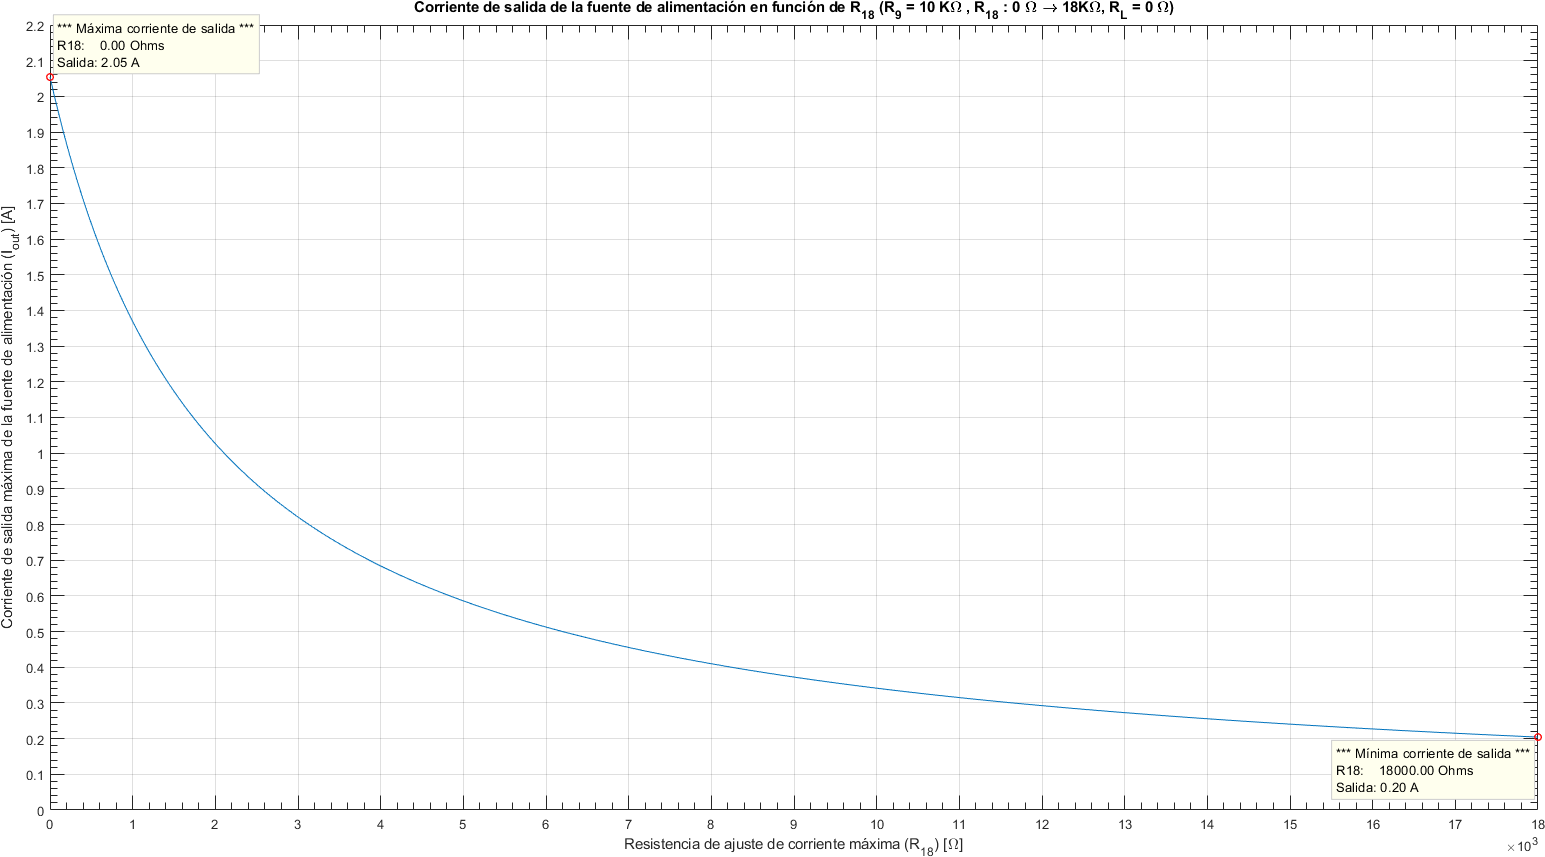
\includegraphics[width=1.2 \textwidth, angle=90]{./img/preguntas/p7.png}
\caption{\label{fig:fig_p7_output_current}\footnotesize{Corriente máxima de salida, $I_{o}$, en función de $R_{18}$, con esta variando entre $0 \si[per-mode=symbol]{\ohm}$ y $18 \si[per-mode=symbol]{\kilo\ohm}$.}}
\end{center}
\end{figure}



\clearpage